\appendix
\addcontentsline{toc}{section}{Appendice}
\section*{Appendices}
\section{Repeatability}
Each variant of the methods was tested with specific seed and initial interval of weight in order to make the execution repeatable.
All network tested with L2 regularization were composed by 1 hidden layer of 15 units.
\begin{table}[H]
	\centering
	\begin{tabular}{|c|c|c|c|c|}
		\hline
		\textbf{Task} &	\textbf{Method} &\textbf{ Variant} & \textbf{Initialization} &\textbf{Seed} \\ \hline
		MONK 1        &    MDA & M  0.6 L2 3e-4 & 1e-2, -1e-2 & 107  \\ \hline
		MONK 2        &    MDA & M  0.6 L2 3e-4 & 1e-2, -1e-2 & 196  \\ \hline
		MONK 3        &    MDA & M  0.6/0.9 L2 3e-4 & 1e-2, -1e-2 & 89  \\ \hline
		MONK 1        &    NMDA & M  0.6 L2 3e-4 & 1e-2, -1e-2 & 70  \\ \hline
		MONK 2        &    NMDA & M  0.6 L2 3e-4 & 1e-2, -1e-2 & 24  \\ \hline
		MONK 3        &    NMDA & M  0.6/0.9 L2 3e-4 & 1e-2, -1e-2 & 31  \\ \hline
		MONK 1        &    PBM  & L2 3e-4 & 1, -1 & 87  \\ \hline
		MONK 2        &    PBM & L2 3e-4 & 1, -1 & 222 *  \\ \hline
		MONK 3        &    PBM & L2 3e-4 & 1e-2, -1e-2 & 33 *  \\ \hline
		MONK 1        &    L-BFGS & L2 3e-4 & 1, -1 & 507  \\ \hline
		MONK 2        &    L-BFGS & L2 3e-4 & 1, -1 & 295  \\ \hline
		MONK 3        &    L-BFGS & L2 3e-4 & 1, -1 & 4  \\ \hline
		
		MONK 1        &    MDA & M  0.6 L1 3e-4 & 1e-2, -1e-2 & 82  \\ \hline
		MONK 2        &    MDA & M  0.6 L1 3e-4 & 1e-2, -1e-2 & 7  \\ \hline
		MONK 3        &    MDA & M  0.6/0.9 L1 3e-4 & 1e-2, -1e-2 & 61  \\ \hline
		MONK 1        &    NMDA & M  0.6 L1 3e-4 & 1e-2, -1e-2 & 82  \\ \hline
		MONK 2        &    NMDA & M  0.6 L1 3e-4 & 1e-2, -1e-2 & 7  \\ \hline
		MONK 3        &    NMDA & M  0.6/0.9 L1 3e-4 & 1e-2, -1e-2 & 61  \\ \hline
		MONK 1        &    PBM & L1 3e-4 & 1e-2, -1e-2 & 4  \\ \hline
		MONK 2        &    PBM & L1 3e-4 & 0, 0 & 30  \\ \hline
		MONK 3        &    PBM & L1 3e-4 & 1e-2, -1e-2 & 33 *  \\ \hline
		MONK 1        &    L-BFGS & L1 3e-4 & 1, -1 & 86  \\ \hline
		MONK 2        &    L-BFGS & L1 3e-4 & 1, -1 & 295  \\ \hline
		MONK 3        &    L-BFGS & L1 3e-4 & 1, -1 & 4  \\ \hline
	\end{tabular}
	\caption{MONK's problems parameter.}
	\label{tab:dati}
\end{table}
* With "percentage\_constraints\_skipped" parameter set to 0.5 of percentage in the algorithm.

\section{Code}
\begin{figure}[H]
	\centering
	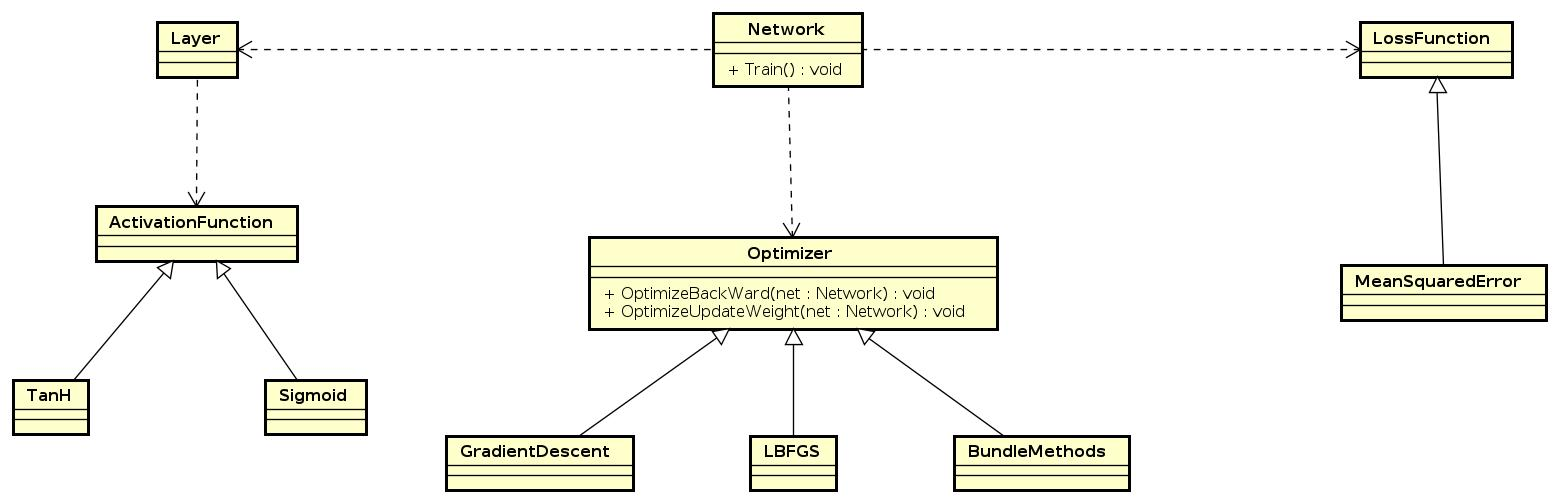
\includegraphics[width=\linewidth]{img/uml.jpg}
	\caption{UML of the project.}
\end{figure}
\newpage